\documentclass{zusammenfassung}
\usepackage{booktabs}
\graphicspath{ {./illustrationen/} }
\usetikzlibrary{shapes.geometric}

\begin{document}

\maketitle{Klasse 6/7}{4. November 2014}{2014/2015}

Eine \emph{Parkettierung} ist eine Überdeckung der Ebene mit Parkettsteinen, wobei keine Lücken zwischen den einzelnen Steinen
bleiben dürfen. Daher ist das keine Parkettierung:

\begin{center}
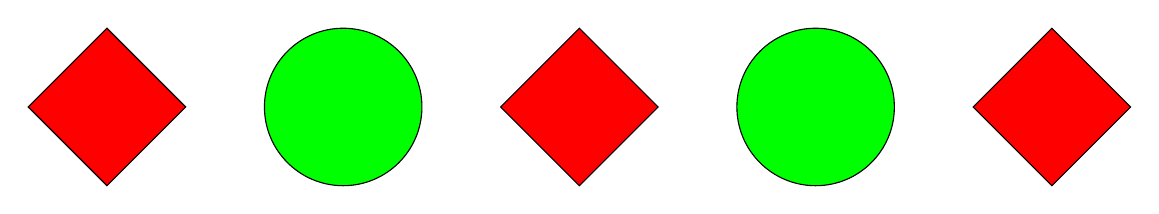
\begin{tikzpicture}
  \draw[fill=red] (0,0) -- (1,1) -- (0,2) -- (-1,1) -- cycle;
  \draw[fill=green] (3,1) circle (1);
  \draw[fill=red] (6,0) -- (7,1) -- (6,2) -- (5,1) --cycle;
  \draw[fill=green] (9,1) circle (1);
  \draw[fill=red] (12,0) -- (13,1) -- (12,2) -- (11,1) --cycle;
\end{tikzpicture}
\end{center}

Um Parkettierungen besser untersuchen zu können, verlangen wir außerdem, dass es nur endlich viele unterschiedliche
Parkettsteine gibt. Wir nennen eine Parkettierung \emph{einfach}, wenn wir nur einen Parkettstein für das ganze Parkett verwenden.

Besonders einfache Parkettsteine sind die \emph{regulären} Polygone oder Vielecke. Das sind Polygone, deren Seiten alle gleich
lang und deren Innenwinkel alle gleich groß sind.

Eine \emph{platonische Parkettierung} ist eine Parkettierung, bei der
\begin{itemize}
  \item[1.] Alle Parkettsteine kongruente reguläre Polygone sind und
  \item[2.] Ecken immer auf Ecken und Seiten immer auf Seiten treffen.
\end{itemize}

\begin{aufgabe}[Beispiele und Nicht-Beispiele von platonischen Parkettierungen]
  \label{aufgabe1}
  Finde jeweils ein Beispiel für eine Parkettierung, die
  \begin{enumerate}
    \item Eigenschaft 1 erfüllt, aber nicht Eigenschaft 2,
    \item Eigenschaft 2 erfüllt, aber nicht Eigenschaft 1,
    \item platonisch ist, also beide Eigenschaften erfüllt.
  \end{enumerate}
\end{aufgabe}

Lösungen zur Aufgabe \ref{aufgabe1} sind in Abbildung \ref{loesung1} dargestellt.

\begin{figure}
  \begin{center}
    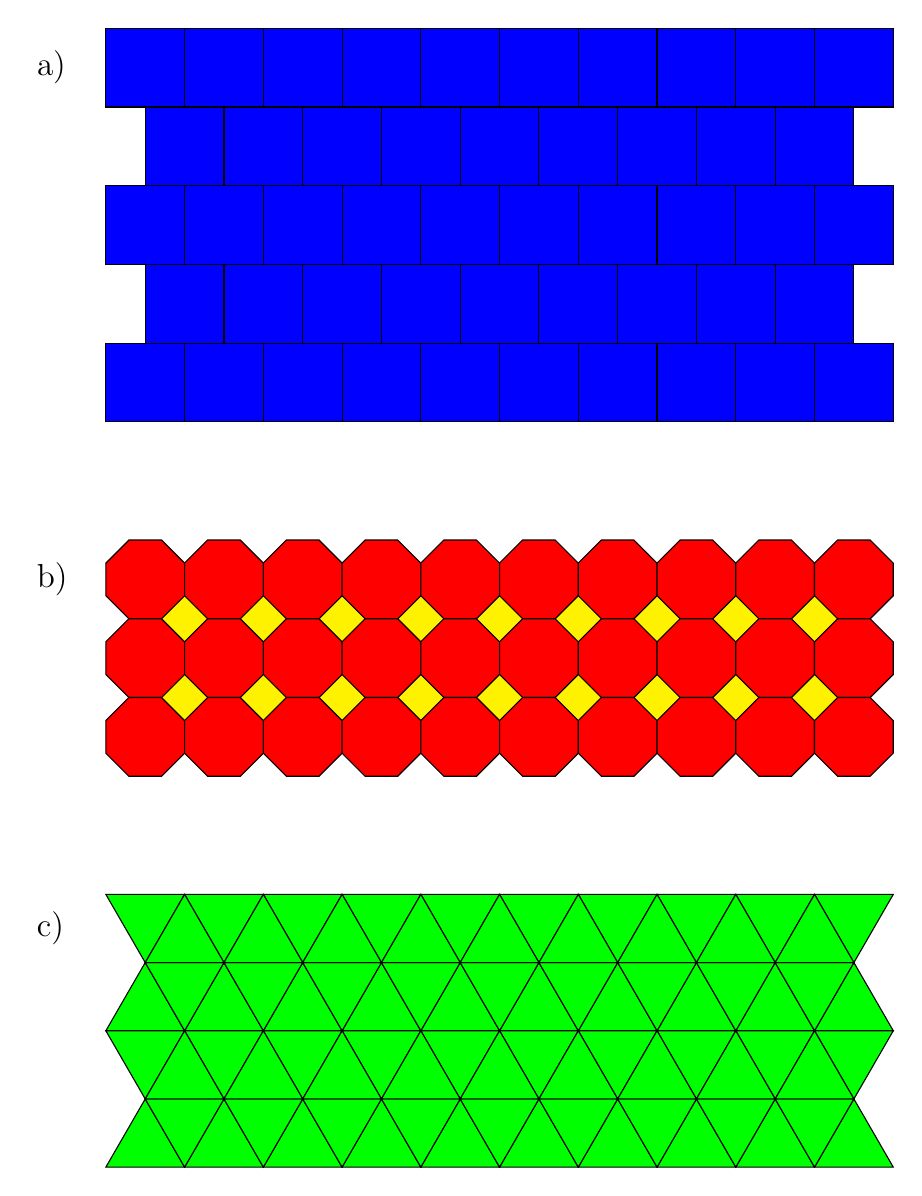
\begin{tikzpicture}[x=1cm,y=-1cm]
      \foreach \i in {1,2,...,10} {
        \draw[fill=blue] (\i,0) rectangle (\i+1,1);
	\draw[fill=blue] (\i,2) rectangle (\i+1,3);
	\draw[fill=blue] (\i,4) rectangle (\i+1,5);
      }
      \foreach \i in {1,2,...,9} {
	\draw[fill=blue] (\i+0.5,1) rectangle (\i+1.5,2);
	\draw[fill=blue] (\i+0.5,3) rectangle (\i+1.5,4);
      }
      \node[anchor=west] at (0,0.5) {\large a)};

      \fill[yellow] (1.5,7) rectangle (10.5,9);
      \foreach \i in {1,2,...,10} {
	\foreach \j in {0,1,2} {
	  \node[draw,fill=red,inner sep=0.3535cm,regular polygon,regular polygon sides=8] at (\i+0.5,\j+7) {};
	}
      }
      \node[anchor=west] at (0,7) {\large b)};

      \foreach \i in {1,2,...,10} {
	\foreach \j in {0,2} {
	  \draw[fill=green] (\i,11+\j*0.866) -- (\i+1,11+\j*0.866) -- (\i+0.5,11.866+\j*0.866) -- cycle;
	  \draw[fill=green] (\i,12.732+\j*0.866) -- (\i+1,12.732+\j*0.866) -- (\i+0.5,11.866+\j*0.866) -- cycle;
	}
      }
      \foreach \i in {1,2,...,9} {
	\foreach \j in {1,3} {
	  \draw[fill=green] (\i+0.5,11+\j*0.866) -- (\i+1.5,11+\j*0.866) -- (\i+1,11.866+\j*0.866) -- cycle;
	  \draw[fill=green] (\i+0.5,11+\j*0.866) -- (\i+1.5,11+\j*0.866) -- (\i+1,10.134+\j*0.866) -- cycle;
	}
      }
      \node[anchor=west] at (0,11.433) {\large c)};

    \end{tikzpicture}
  \end{center}
  \caption{Beispielhafte Lösungen zu Aufgabe 1}
  \label{loesung1}
\end{figure}

Wir wollen herausfinden, welche verschiedenen platonischen Parkettierungen es gibt. Dazu betrachten wir eine Ecke des Parketts:

\begin{center}
  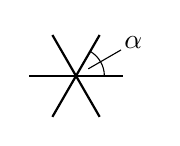
\begin{tikzpicture}[scale=0.6]
    \foreach \i in {0,60,120,...,300} {\draw[thick] (0:0) -- (\i:1);}
    \draw (0:0.6) arc (0:60:0.6);
    \draw (30:0.3) -- (30:1.1) (30:1.4) node[anchor=mid] {$\alpha$};
  \end{tikzpicture}
\end{center}

\pagebreak
Alle Winkel, die an der Ecke zusammentreffen, sind Innenwinkel von kongruenten regulären Polygonen und damit alle gleich groß.
Das bedeutet, dass der Vollwinkel, also die Summe alle Winkel an der Ecke, ein Vielfaches des Innenwinkels $\alpha$ sein muss.
Der Vollwinkel beträgt $360^\circ$.

\begin{aufgabe}[Innenwinkel im regulären Vieleck]
  Wie groß sind Winkelsumme und Innenwinkel im regulären Drei-, Vier-, Fünf-, Sechs-, Sieben- und Achteck?
\end{aufgabe}

Eine Möglichkeit, diese Aufgabe zu lösen, ist, die Vielecke in Dreiecke zu zerlegen:

\begin{center}
  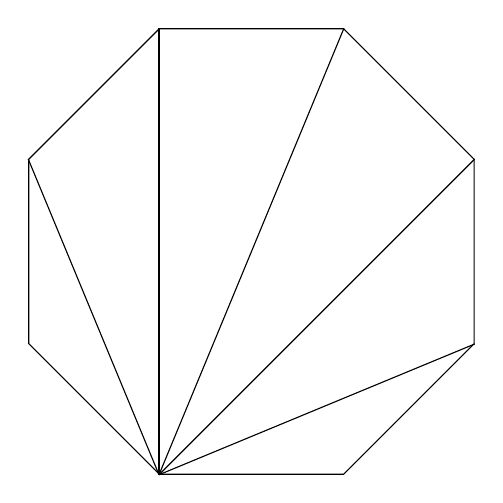
\begin{tikzpicture}
    \node[draw,inner sep=2cm,regular polygon,regular polygon sides=8] (a) at (0,0) {};
    \foreach \i in {1,2,3,7,8} {\draw[fill=black] (a.corner 5) -- (a.corner \i);}
  \end{tikzpicture}
\end{center}

Jedes der Dreiecke hat die Winkelsumme $180^\circ$, und die Anzahl der Dreiecke, die man erhält, ist um $2$ kleiner als die
Anzahl der Ecken des Vielecks. Daher erhalten wir die Formel
\[
  \text{Winkelsumme im regulären Vieleck}=(\text{Anzahl der Ecken des Vielecks}-2)\cdot 180^\circ.
\]
Da jeder Winkel gleich groß ist, ist also die Größe eines Innenwinkels gegeben durch den Quotient aus der Winkelsumme mit der
Anzahl der Ecken, also
\[
  \text{Größe eines Innenwinkels}=\frac{(\text{Anzahl der Ecken}-2)\cdot 180^\circ}{\text{Anzahl der Ecken}}.
\]

Daher erhalten wir die folgenden Ergebnisse für die Drei- bis Achtecke:

\begin{center}
  \begin{tabular}{ccc}
    \toprule
    \textbf{Anzahl der Ecken}&\textbf{Winkelsumme}&\textbf{Innenwinkel}\\
    \midrule
    $3$&$180^\circ$&$60^\circ$\\
    $4$&$360^\circ$&$90^\circ$\\
    $5$&$540^\circ$&$108^\circ$\\
    $6$&$720^\circ$&$120^\circ$\\
    $7$&$900^\circ$&$\approx 129^\circ$\\
    $8$&$1080^\circ$&$135^\circ$\\
   \bottomrule
  \end{tabular}
\end{center}

Teiler von $360^\circ$ sind $180^\circ$, $120^\circ$ oder kleiner. $180^\circ$ kann als Innenwinkel nicht auftauchen, und
alle Vielecke mit mehr als sieben Ecken haben größere Innenwinkel als $120^\circ$. Außerdem ist der Innenwinkel des Fünfecks
offenbar ebenfalls kein Teiler von $180^\circ$. Das heißt, dass für platonische Parkette nur noch Drei-, Vier- und Sechsecke
als Parkettsteine in Frage kommen. Das Parkett aus Dreiecken wurde schon in der Lösung zu Aufgabe \ref{aufgabe1} abgebildet,
und man findet auch Parkette aus regulären Vier- beziehungsweise Sechsecken:

\begin{center}
  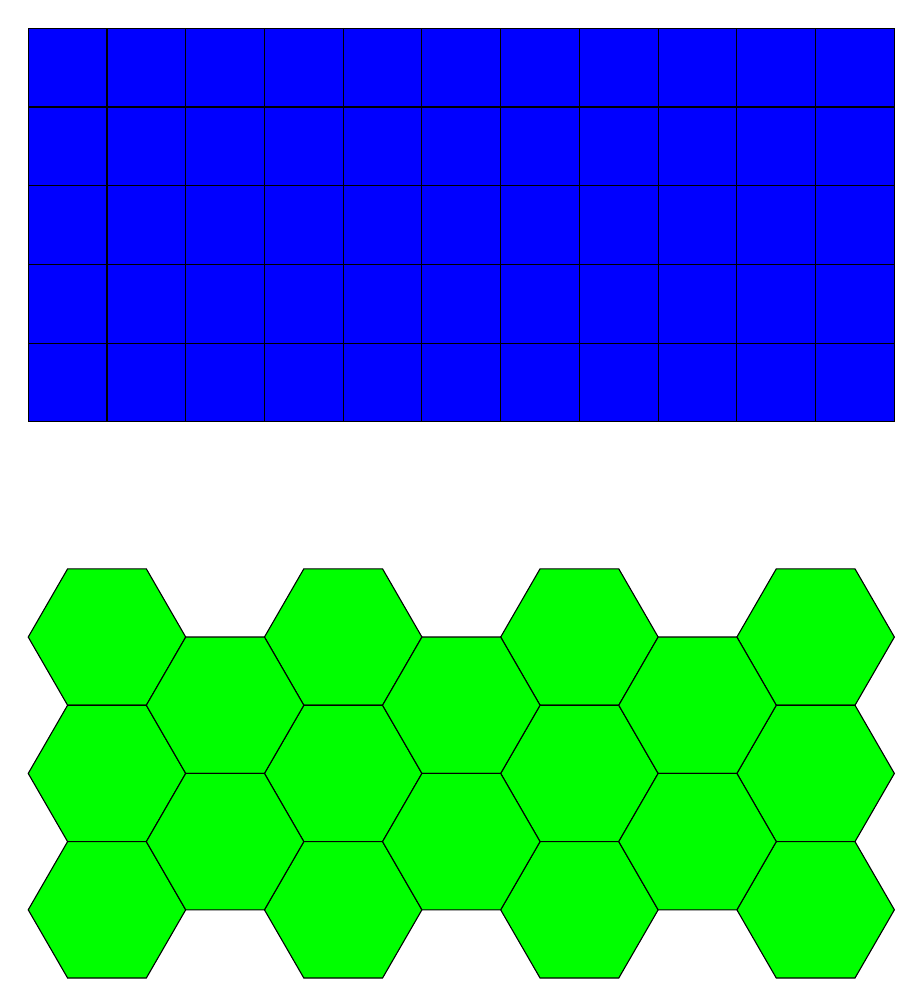
\begin{tikzpicture}[x=1cm,y=-1cm]
    \foreach \i in {1,2,...,11} {
      \draw[fill=blue] (\i,0) rectangle (\i+1,1);
      \draw[fill=blue] (\i,1) rectangle (\i+1,2);
      \draw[fill=blue] (\i,2) rectangle (\i+1,3);
      \draw[fill=blue] (\i,3) rectangle (\i+1,4);
      \draw[fill=blue] (\i,4) rectangle (\i+1,5);
    }
    \foreach \j in {1,2,3} {
      \foreach \k in {0,1,...,3} {
        \draw[fill=green,shift={(2+3*\k,6+\j*1.732)}] (0:1) \foreach \i in {60,120,...,300} {-- (\i:1) } -- cycle;
      }
    }
    \foreach \j in {1,2} {
      \foreach \k in {0,1,2} {
        \draw[fill=green,shift={(3.5+3*\k,6.866+\j*1.732)}] (0:1) \foreach \i in {60,120,...,300} {-- (\i:1) } -- cycle;
      }
    }
  \end{tikzpicture}
\end{center}

Platonische Parkettierungen sind sehr regelmäßige Parkettierungen. Die sogenannten \emph{Penrose-Parkettierungen}
zeigen, dass man auch auf eine unregelmäßige Art mit wenigen Teilen die Ebene parkettieren kann. Auf der nächsten Seite finden
sich Vorlagen, die man ausdrucken und aneinanderlegen kann. Dabei müssen wieder Ecken auf Ecken und Kanten auf Kanten treffen,
und außerdem müssen die Kreislinien aufeinanderpassen. Das Parkett, das sich dann bildet, hat eine Fünfeckssymmetrie, 
aber im Gegensatz zu den platonischen Parketten ist es nicht \emph{translationsinvariant}: Man erhält nicht durch Verschieben
dasselbe Muster zurück.

\pagebreak
\newgeometry{top=1cm,bottom=1cm}
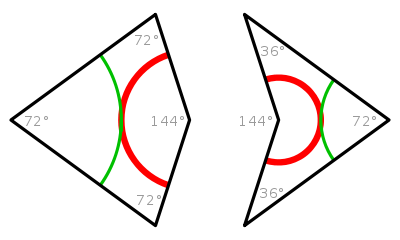
\includegraphics[width=0.45\textwidth]{penrose_kite_dart.png}
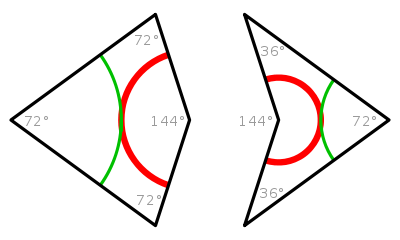
\includegraphics[width=0.45\textwidth]{penrose_kite_dart.png}\\[0.2cm]
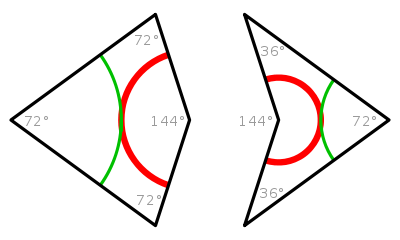
\includegraphics[width=0.45\textwidth]{penrose_kite_dart.png}
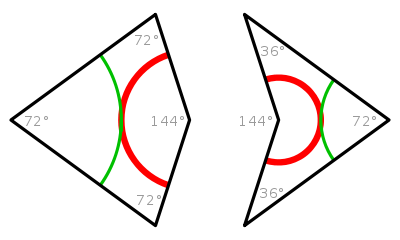
\includegraphics[width=0.45\textwidth]{penrose_kite_dart.png}\\[0.2cm]
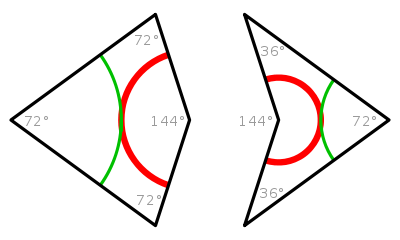
\includegraphics[width=0.45\textwidth]{penrose_kite_dart.png}
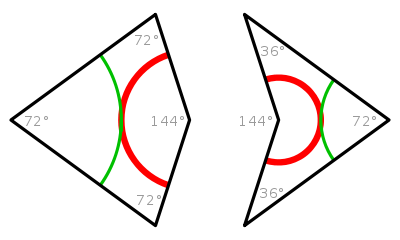
\includegraphics[width=0.45\textwidth]{penrose_kite_dart.png}\\[0.2cm]
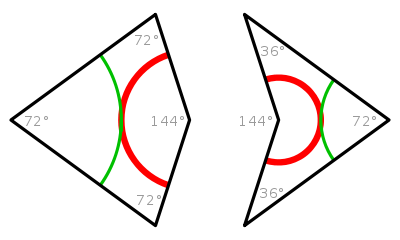
\includegraphics[width=0.45\textwidth]{penrose_kite_dart.png}
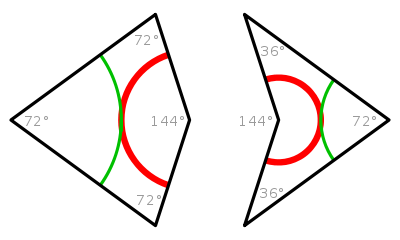
\includegraphics[width=0.45\textwidth]{penrose_kite_dart.png}\\[0.2cm]
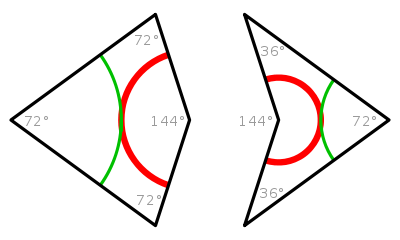
\includegraphics[width=0.45\textwidth]{penrose_kite_dart.png}
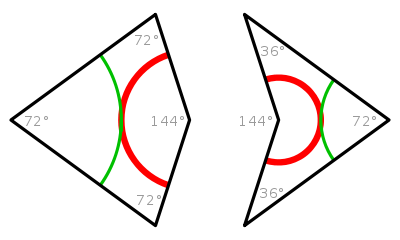
\includegraphics[width=0.45\textwidth]{penrose_kite_dart.png}\\[0.2cm]
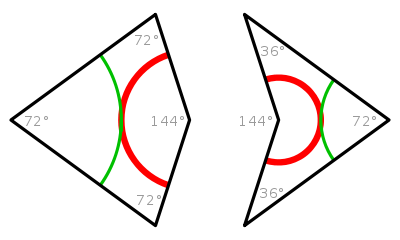
\includegraphics[width=0.45\textwidth]{penrose_kite_dart.png}
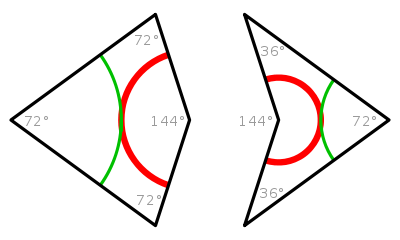
\includegraphics[width=0.45\textwidth]{penrose_kite_dart.png}

\end{document}
